\documentclass[a4paper, oneside]{discothesis}

% use utf8 instead of latin1 when using LaTeX in windows
\usepackage[latin1]{inputenc}
\usepackage{listings}
\usepackage{subcaption}
\usepackage{graphicx}
\usepackage{caption}

\lstset{ %
	language=C++,
	keepspaces=true, 
	numbers=left, 
	basicstyle=\footnotesize, 
	numberstyle=\footnotesize, 
	tabsize=2,
	frame=single
	} 


%%%%%%%%%%%%%%%%%%%%%%%%%%%%%%%%%%%%%%%%%%%%%%%%%%%%%%%%%%%%%%%%%%%%%%%%%%%%%%%%%%%%%%%%%%%%%%%%%
% DOCUMENT METADATA

\thesistype{Bachelor Thesis}
\title{3D Depth Sensor on Mobile Devices \\ \large Acquisition, Calibration and 3D Reconstruction}

\author{Lukas Bischofberger}
\email{lukasbi@ethz.ch}
\institute{Computer Vision and Geometry Group \\[2pt]
Institute for Visual Computing \\[2pt]
ETH Z�rich}

% You can put in your own logo here "\includegraphics{...}" or just comment the command
%\logo{}
%
\includegraphics{figures/cvg.png}

\supervisors{Dr. Amael Delaunoy\\[2pt] Prof.\ Dr.\ Marc Pollefeys}

% You can comment the following two commands if you don't need them
% \keywords{Keywords go here.}
% \categories{ACM categories go here.}

\date{\today}

%%%%%%%%%%%%%%%%%%%%%%%%%%%%%%%%%%%%%%%%%%%%%%%%%%%%%%%%%%%%%%%%%%%%%%%%%%%%%%%%%%%%%%%%%%%%%%%%%

\begin{document}

\frontmatter % do not remove this line
\maketitle

\cleardoublepage

\begin{acknowledgements}
	I would like to thank my supervisor Amael Delaunoy for his support and great help I received during the weekly meetings. I also want to thank Professor Marc Pollefeys for offering me the opportunity to write my bachelor thesis at the Computer Vision and Geometry Group.
\end{acknowledgements}


\begin{abstract}
	The introduction of Kinect has made depth sensors available to the consumer world. This made it possible for basically everyone to have a 3D scanner at home. Systems like Kinect Fusion would give the possibility to easily get a 3D reconstruction of everything in front of the lens. 
	
	The structure sensor by Occipital is the first mobile depth sensor and thus brings the possibility to have a mobile 3D scanner. We want to show that mobile depth data acquisition is possible and easy and also that this data performs well in 3D reconstruction applications.
	\newline
	Therefore a pipeline from data acquisition on a mobile device up to 3D reconstruction on a desktop computer has been developed.  
\end{abstract}

\setcounter{tocdepth}{1}
\tableofcontents

\mainmatter % do not remove this line

% Start writing here

\chapter{Introduction}
	We want to use a state of the art mobile device for depth data acquisition. For this we take advantage of the first mobile depth sensor, the Structure sensor by Occipital\footnote{https://occipital.com/}. Further we will combine the depth sensor with the color camera of the device for texturing a 3D model.

	We want to show that this data can then be used to create a 3D reconstruction. For this step we will use camera tracking and motion estimation algorithms and another pipeline for volumetric mapping.
	
	\section{Motivation}
		We want to show that with mobile devices like smartphones or a tablets, which today are omnipresent and a fairly low cost sensor we can perform 3D scanning. This scans could be used in numerous applications in daily life. 
		
		Scans of rooms can for example be used to measure their dimensions and check for furniture to fit in. This is partly implemented in the IKEA Catalog application, whereas there no real measurements and room structure are available\footnote{https://play.google.com/store/apps/details?id=com.ikea.catalogue.android}. On the other hand such a scan could also be used for real estate advertisements, e.g. by showing reconstructed interiors depicted with real dimensions. In general every reconstructed object could also be printed by a 3D printer. A last intention is also to show that 3D reconstruction with depth data performs better and faster than such with color images only.
		
	\newpage

	\section{Contribution}
		The contributions of our work are the following:
		
			\begin{itemize}
				\item An iOS application for the depth and color data acquisition which is based on the Structure SDK\footnote{Software development kit}\footnote{http://structure.io/developers}. It allows viewing and recording of RGB-D\footnote{RGB color space with an added depth channel} data as well as camera calibration.
				\item An offline pipeline which consists of two parts. The first part will convert the raw data recorded on the mobile device to RGB-D pairs using the calibration results. The second part estimates the camera motion and performs a 3D reconstruction.
			\end{itemize}
	
	\section{Related work}
		There have been different approaches on reconstruction, ranging between professional solutions, to consumer accessible products up to research projects. They also differ on their technical approach.  NextEngine for example uses high precision laser scanning and KinectFusion uses its proper sensor which is a combination of different cameras. The third approach described here solely relies on color images. 
		
		\subsection{Kinect Fusion}
			Kinect Fusion \cite{...} is an application which provides 3D scanning and model creation based on the Kinect sensor\footnote{https://msdn.microsoft.com/en-us/library/dn188670.aspx}. The Kinect sensor is a horizontal bar which features a RGB camera, a depth sensor and a multi-array microphone\footnote{http://blog.seattlepi.com/digitaljoystick/2009/06/01/e3-2009-microsoft-at-e3-several-metric-tons-of-press-releaseapalloza/}. The user can paint a scene with the Kinect camera and simultaneously see, and interact with, a detailed 3D model of the scene. Kinect Fusion runs on a Desktop PC with the sensor attached by wire. The reconstruction and estimation of the camera movement is based on the tracking of the camera through the depth map. Further there exist possibilities to color the constructed models or to apply shading.
			
		\subsection{Live Metric 3D Reconstruction on Mobile Phones}
			A paper by Tanskanen et al. \cite{paper1} proposes a complete on-device approach for 3D reconstruction. It uses a monocular hand-held device without any depth sensor. The reconstruction process is solely based on color images but the camera motion estimation takes advantage of the device own inertial sensors. Furthermore the paper proposes an efficient and accurate multi-resolution scheme for dense stereo matching which takes into account the restricted computational capabilities of the mobile device.
			
		\subsection{3D Scanner}
			In the industry products like NextEngine 3 Scanner\footnote{http://www.nextengine.com/} have been available for some time. This scanner has a laser for high precision scanning and thus obtains far higher quality models than the approaches described before. It also features export to industry standard applications and allows easy printing of the scans. On the other side special equipment is needed which is considerably more expensive than consumer electronic devices.
			
		\subsection{Structure Sensor}	
			Our approach is different insofar that we use generally available hardware as the iPad's color camera and an affordable depth sensor. However our data is quite similar to that of \cite{kinect} with the difference that the data capturing is entirely done on a mobile device. In theory the reconstruction could also be done on the mobile device as described in chapter 5.

\chapter{Data Acquisition}

	\footnotetext[1]{http://structure.io/developers}

	In this chapter we give a detailed description on how the data acquisition on a mobile device is performed. In a first step we describe the use of the Structure sensor, it's mechanism and how we obtain the data in a meaningful way. Then we describe the relation between the depth data and color images taken from the device camera. In a third step we will show how to perform camera calibration and combine the data to RGB-D image pairs. 

	\section{Mobile Depth Acquisition}
		The Structure sensor is a so called structured-light 3D scanner. It possesses an infrared structured light projector and a corresponding camera system\footnotemark[1]. The projector projects an infrared mesh onto the scene, which the camera records from a slightly different angle. The three-dimensionally shaped surface produces a distorted mesh relative to the viewing camera, which is then able to perform a geometric reconstruction of the surface shape.
		
		\begin{figure}[h]
			\centering
			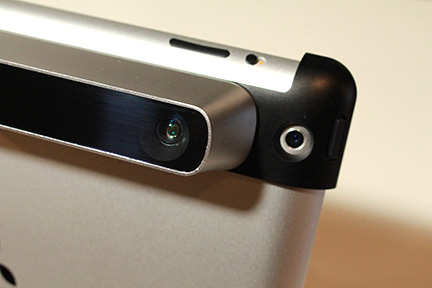
\includegraphics[width=0.75\textwidth]{figures/ipad-sensor}
%			\footnote{http://structure.io/static/occipital/images/v1/getstarted/ipad\_camera\_centered.jpg}
			\caption{Structure sensor on the iPad \ref{img:sensor}}
			\label{fig:sensor}
		\end{figure}

		The sensor is connected to the device by cable, in our case to the iPad through the lightning port. We use the Structure SDK\footnotemark[1] as an interface between our application and the sensor hardware. This allows us to receive depth frames or infrared images at different scales. Unfortunately the maximum resolution of the depth sensor is only 640x480 pixels. Additionally, the SDK provides the possibility to get synchronized infrared/color or depth/color pairs. The color images are taken by the mobile device's own camera, e.g. the iPad's camera through the AVFoundation framework\footnote{https://developer.apple.com/library/mac/documentation/AVFoundation/Reference/
		AVFoundationFramework/index.html}. 
		
		Originally we wanted to perform the mobile data acquisition on an Android device. This had the advantage that we could rely on standard libraries like OpenNI \footnote{http://structure.io/openni} and OpenCV \footnote{http://opencv.org/}. The drawback was that applications on Android are written in Java and the C++ libraries are only accessible through the native development kit (NDK) \footnote{https://developer.android.com/tools/sdk/ndk/index.html} interface. Unfortunately we weren't able to make the structure sensor work on this platform, thus we decided to work on the iOS platform where a SDK for the sensor was provided.
		
		\begin{figure}[h]
			\centering
			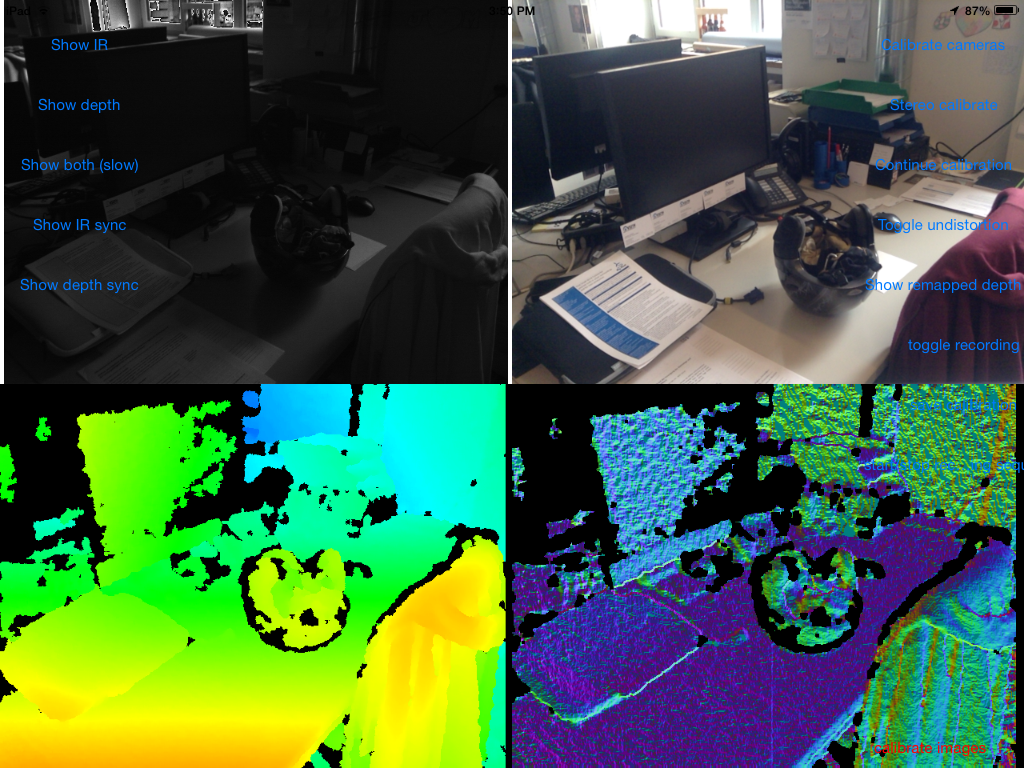
\includegraphics[width=0.75\textwidth]{figures/acquisition}
			\caption{Data acquisition screen}
			\label{fig:acquisition}
		\end{figure}
		
		On the data acquisition screen (Figure \ref{fig:acquisition}) we see the infrared image on the top left, the color image on the top right, the depth map on the bottom left, whereas red/yellow pixels indicate a close location and blue/black pixels represent the far away areas. Finally we can also see the surface normals on the bottom right.
		

	\section{RGB and Depth Camera Calibration}

		For the camera calibration we make use of the pinhole camera model which will briefly be explained here. The next section describes how the depth sensor and the device's RGB camera are calibrated. This will provide the camera matrices and lens distortion coefficients for both cameras. After the single camera calibration for both cameras, the third section explains how these results can be used to perform a stereo camera calibration, which finds the extrinsic parameters. 
		
		\subsection{Pinhole Camera Model}
		
			The pinhole camera model\footnote{http://docs.opencv.org/modules/calib3d/doc/camera\_calibration\_and\_3d\_reconstruction.html} describes the mapping of a 3D point to a 2D image. Equation \ref{eq:model} explains the basic relationship between a 3D point and its projection onto the image plane by using perspective transformation.
			
			\begin{equation}
				s p = K(RP + t)
				\label{eq:model}
			\end{equation}
			
%			\begin{pmatrix}X\\Y\\Z\end{pmatrix}

			Here $P = (X,Y,Z)^T$ is a 3D point in the world coordinate space and $p = (u,v,1)^T$ is the projection of $P$ in the camera frame in pixels.
			
			\begin{equation}
				K =
				\begin{bmatrix}
					f_x & 0 & c_x\\
					0 & f_y & c_y\\
					0 & 0 & 1
				\end{bmatrix}
				\label{eq:K}
			\end{equation}
						
			$K$ is called the camera matrix or a matrix of intrinsic parameters, $f_x, f_y$ are the focal lengths expressed in pixel units and $(c_x,c_y)$ is the principal point which is usually located at the image center. Furthermore we have the rotation matrix
			
			\begin{equation}
			R =
			\begin{bmatrix}
			r_{11} & r_{12} & r_{13}\\
			r_{21} & r_{22} & r_{23}\\
			r_{31} & r_{32} & r_{33}
			\end{bmatrix}
			\label{eq:R}
			\end{equation}
			
			 and the translation vector 
			 
			 \begin{equation}
			 		t=
			 			\begin{bmatrix}
			 				t_1\\
			 				t_2\\
			 				t_3
			 			\end{bmatrix}.
			 			\label{eq:t}
			 		\end{equation}
			 		
			 		We will refer to $[R|t]$ as the matrix of extrinsic parameters. It is used to describe the camera motion around a static scene. In a more general application the extrinsic parameters also describe the rigid motion of an object in front of a stationary camera.  
			 		
			\begin{figure}[h]
				\centering
				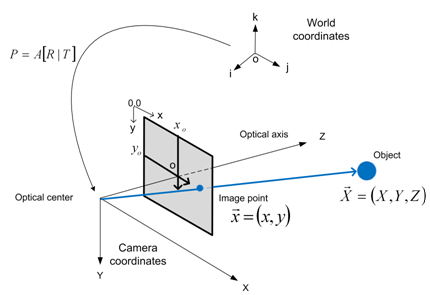
\includegraphics[width=0.75\textwidth]{figures/pinhole}
				\footnote{http://archimede.bibl.ulaval.ca/archimede/fichiers/25229/25229\_35.png}
				\caption{Pinhole camera model}
				\label{fig:pinhole}
			\end{figure}
			
%			\newpage
			
			Real lenses usually have some radial and tangential distortion. To account for this the distortion coefficients $k_1$ to $k_6$ and $p_1$ and $p_2$ are introduced and the camera model is extended as follows.
			
			\begin{equation}
				\begin{pmatrix}x\\y\\z\end{pmatrix} = R \begin{pmatrix}X\\Y\\Z\end{pmatrix} + t
			\end{equation}
			\begin{equation}
				x' = \frac{x}{z}, y' = \frac{y}{z}
			\end{equation}
			\begin{equation}
				\begin{split}
					x'' = x'\frac{1 + k_1 r^2 + k_2 r^4 + k_3 r^6}{1 + k_4 r^2 + k_5 r^4 + k_6 r^6} + 2 p_1 x' y' + p_2(r^2 + 2 x'^2)  \\ 
					y'' = y'\frac{1 + k_1 r^2 + k_2 r^4 + k_3 r^6}{1 + k_4 r^2 + k_5 r^4 + k_6 r^6} + p_1 (r^2 + 2 y'^2) + 2 p_2 x' y'  \\
					\text{where} \quad r^2 = x'^2 + y'^2  \\
				\end{split}
			\end{equation}
			\begin{equation}
				\begin{split}
						u = f_x*x'' + c_x \\ v = f_y*y'' + c_y
				\end{split}
			\end{equation}
			
			\begin{figure}[h]
				\centering
				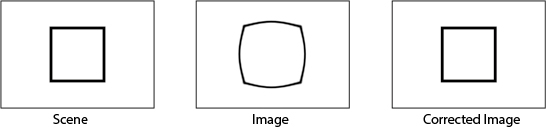
\includegraphics[width=0.75\textwidth]{figures/distortion}
				\footnote{}
				\caption{Distortion}
				\label{fig:distortion}
			\end{figure}
		
		\subsection{Single Camera Calibration}
			We record a set of images of a specific pattern from different viewpoints to do the camera calibration. We choose a chessboard pattern which is a standard choice for calibration because corners can easily be detected. A corner detection algorithm can search for a specified amount of corners, which are the projection of the scene points on the image plane. Because we assume a chessboard we know the location of the corners in a respective coordinate system (which is assumed to be the world coordinate system for the calibration). Accordingly we have several images and thus several equations and we can solve for \ref{eq:model} and find \ref{eq:K}, \ref{eq:R} and \ref{eq:t}.  
			
			Furthermore the calibration process will also find the distortion coefficients by minimizing
			
			\begin{equation}
				f(k_1,k_2,...) = \sum_{i}^{} (x'_i-x_{ci})^2 + (y'_i-y_{ci})^2
			\end{equation}
			
			where 
			
			\begin{equation}
				\begin{split}
					x_{c} - x_0 = L(r)(x-x_0) \\
					y_{c} - y_0 = L(r)(y-y_0)
				\end{split}
			\end{equation}
			
			and 
			
			\begin{equation}
				L(r) = 1 + k_1r+k_2r^2+...
			\end{equation}
			
			\begin{figure}[h]
				\centering
				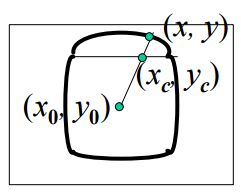
\includegraphics[width=0.2\textwidth]{figures/pixel_undist}
				\caption{Undistortion}
				\label{fig:calib}
			\end{figure}			
			
			
			We do this calibration separately for the color camera and the infrared sensor. Typically a good calibration has a RMS of the back-projection error of about 0.1 to 1 pixels. We obtained a RMS of around 0.2 pixels for the color camera and a little worse result of about 1.2 pixels for the infrared sensor. We were able to keep the error low by for example fixing the principal point of the image. 
			
			We know found the camera matrix and the distortion coefficients for both cameras. In our case this is only an intermediate result, we will continue with the stereo calibration where the single camera calibration results can be used as input parameters.
		
			
			\begin{figure}[h]
				\centering
				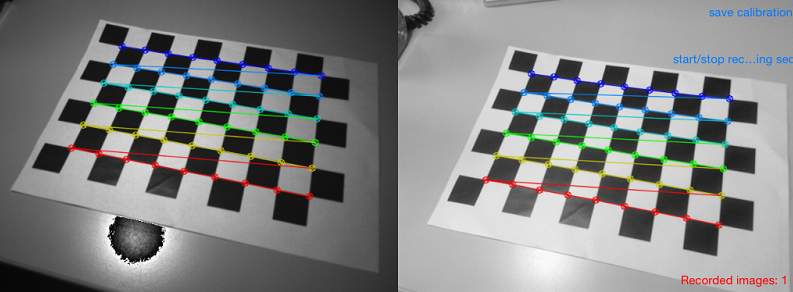
\includegraphics[width=0.75\textwidth]{figures/calib1}
				\caption{IR and RGB images with the calibration pattern}
				\label{fig:calib}
			\end{figure}
			
			\begin{figure}[h]
				\centering
				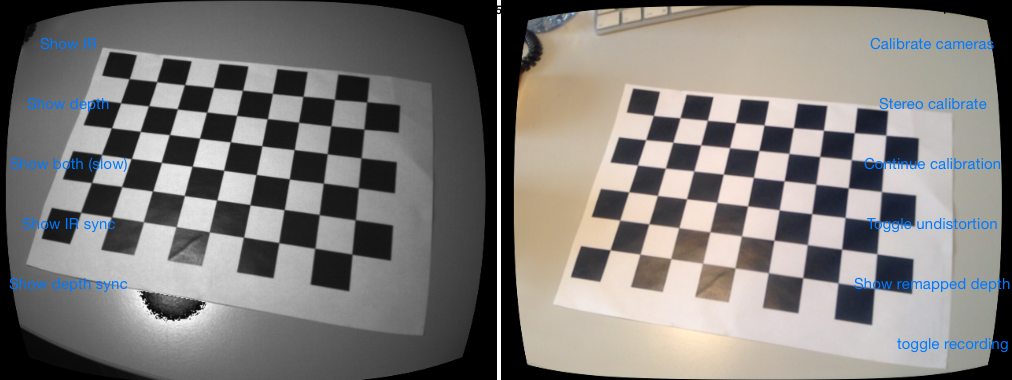
\includegraphics[width=0.75\textwidth]{figures/undist}
				\caption{Undistorted IR and RGB images}
				\label{fig:undist}
			\end{figure}
			
			\todo{better images}
		
		\subsection{Stereo Calibration}
			In the stereo calibration the extrinsic parameters are estimated. We want to find the rotation and translation between the two camera centers. We will use the precomputed camera matrices and intrinsic parameters from the previous section as well as synchronized RGB-D pairs as input. 
			
			Stereo correspondence is usually found using epipolar geometry. Two cameras recording the same scene from different viewpoints span the epipolar plane. It is bounded by the line from the camera center $c_0$ through the projection of p onto the image plane to p and vice versa for camera center $c_1$. The third bounding line is the connection between the two camera centers through the epipoles $e_0$ and $e_1$. Along that, we get a pair of epipolar lines which are the line segments $x_0$ to $e_0$ and $x_1$ to $e_1$, extended to infinity. 
			
			\begin{figure}[h]
				\centering
				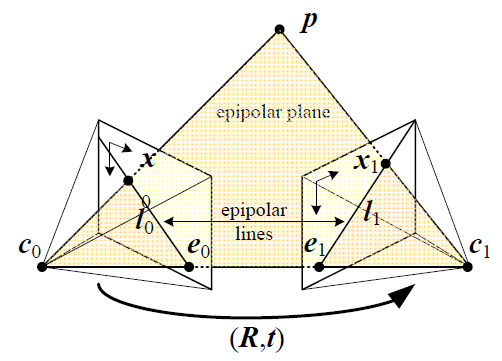
\includegraphics[width=0.75\textwidth]{figures/epipolar}
				\caption{Epipolar geometry}
				\label{fig:epipolar}
			\end{figure}			
			
			The epipolar lines are the intersection of the image planes with the epipolar plane. Then using the epipolar constraint we can define the essential matrix
			
			\begin{equation}
				E = [t]_{\times}R
			\end{equation} 
			which can be used to recover the camera motion. The exact procedure is omitted here but using several images it is possible to compute the rotation matrix $R$ and translation vector as described in  $t$ \cite{cvbook}.		
			
%			\begin{figure}[h]
%				\centering
%				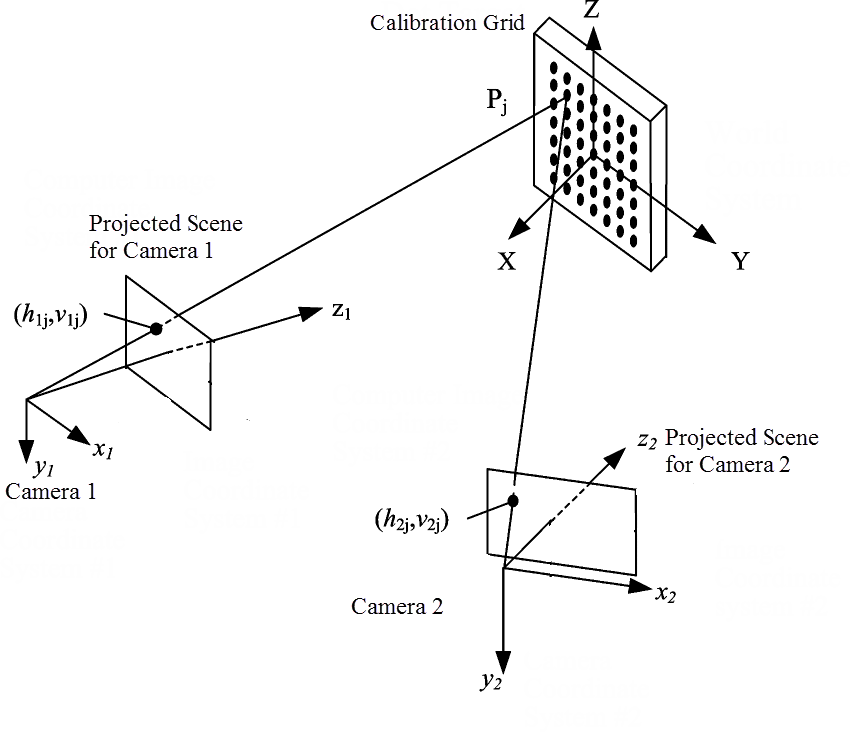
\includegraphics[width=0.8\textwidth]{figures/stereo}
%				\caption{Stereo camera calibration}
%				\label{fig:stereo}
%			\end{figure}
			
%			For better understanding we can also represent $R$ and $t$ as a combination of two camera to world  transformations.
%			
%			\begin{equation}
%				R = R_{rgb}(R_{ir})^{T}
%			\end{equation}
%			
%			\begin{equation}
%			t = t_{rgb} + Rt_{ir}
%			\end{equation}
%			
%			Where $R_{rgb}$ and $t_{rgb}$ are the extrinsic parameters of the color camera and vice versa for the infrared camera. Thus $R$ and $t$ define the transformation from the infrared coordinate system to the color camera coordinate system.
			
			The algorithm uses the calibration points obtained before to construct the epipolar plane. Furthermore we pass the intrinsics computed in the previous single camera calibration as input to reduce the dimension of the parameter space. Additionally flags can be passed to the algorithm, e.g. to fix the intrinsics, to further restrict the solution. The quality of the stereo calibration can be controlled by looking at the RMS like in the single camera calibration. Here the error is usually a little higher but values between 0.5 and 1.5 pixels yielded good results.
						
%			\begin{equation} \label{eq:prgb}
%				P_{rgb} = R_{rgb} * p_{rgb} + t_{rgb}
%			\end{equation}
%			
%			\begin{equation} \label{eq:pir}
%				p_{ir} = R_{ir} * P_{ir} + t_{ir}
%			\end{equation}
%			
%%			Combining \ref{eq:prgb} and \ref{eq:pir} will leave us with
%			Hence we get the rotation matrix and the translation vector between the two camera centers. 
%			
%			\begin{equation}
%				R = R_{ir}(R_{rgb})^{T}, t = t_{ir} + Rt_{rgb}
%			\end{equation}			
%			
%			\begin{equation}
%				p_{rbg} = K_{rgb} * R * K_{ir}^{-1} * p_{ir} + t 
%			\end{equation}

%	\TODO{side by side of rectified image pair?}
		
	\section{Depth re-projection}
		The last step in the data acquisition is to use the results obtained in the previous steps and re-project the depth onto the color image. Thus we want to create an RGB-D pair with depth and color information.  For storage reasons we will not create a four channel image but use a three channel RGB and a single channel depth image.
		
		From now on, instead of recording infrared/color image pairs, we record depth/color pairs. It must be ensured that the sensor is fixed at the same position relative to the color camera as with which the calibration was performed. The algorithm in \ref{ap:reprojection} is used alongside with the calibration results to project every pixel in the depth frame to its corresponding location in the color camera image plane.
		
		For every pixel $p_{depth}$ this is done as follows, first we project it into its cameras coordinate system using the respective camera matrix (\ref{eq:todepthsystem}). Then we apply the rotation and translation obtained during stereo calibration to $P_{depth}$ to transform the point into the color camera coordinate system (\ref{eq:Prgb}). And last we back-project the point $P_{rgb}$ into the color camera frame to obtain its pixel coordinates using the color camera matrix (\ref{eq:prgb}). Besides the $z$ coordinate of the point in the color camera coordinate system represents the depth of $p_{rgb}$ (\ref{eq:prgbdepth}).
		
		Mathematically this procedure can be formulated in the following way:   
		\begin{equation}
			\label{eq:todepthsystem}
			P_{depth} = K_{ir}^{-1}\cdot p_{depth}
		\end{equation}
		
		\begin{equation}
			\label{eq:Prgb}
			P_{rgb} = R \cdot P_{depth} + t
		\end{equation}
		
		\begin{equation}
			\label{eq:prgb}
			p_{rgb} = K_{rgb}\cdot P_{rgb}
		\end{equation}
		
		\begin{equation}
			\label{eq:prgbdepth}
			\text{depth of } p_{rgb} = P_{rgb}.z
		\end{equation}
		
%		\begin{figure}[h]
%			\centering
%			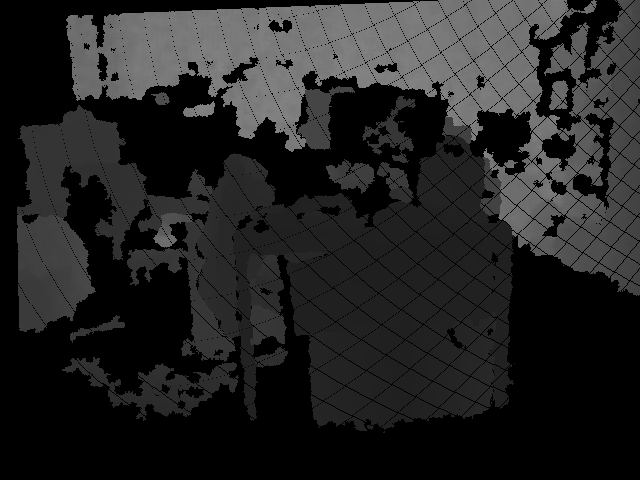
\includegraphics[width=0.75\textwidth]{figures/reprojection}
%			\caption{Re-projected depth image}
%			\label{fig:reprojection}
%		\end{figure}
		
		\begin{figure}[h]
			\centering
			\begin{subfigure}[b]{0.3\textwidth}
				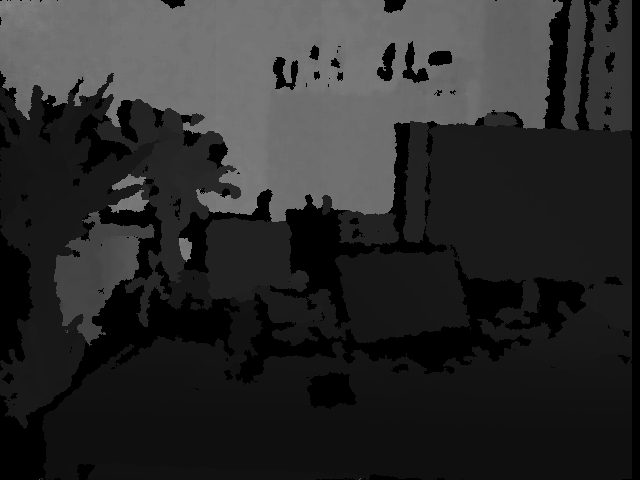
\includegraphics[width=\textwidth]{figures/depth1}
				\caption{Depth frame}
				\label{fig:depth1}
			\end{subfigure}
			~
			\begin{subfigure}[b]{0.3\textwidth}
				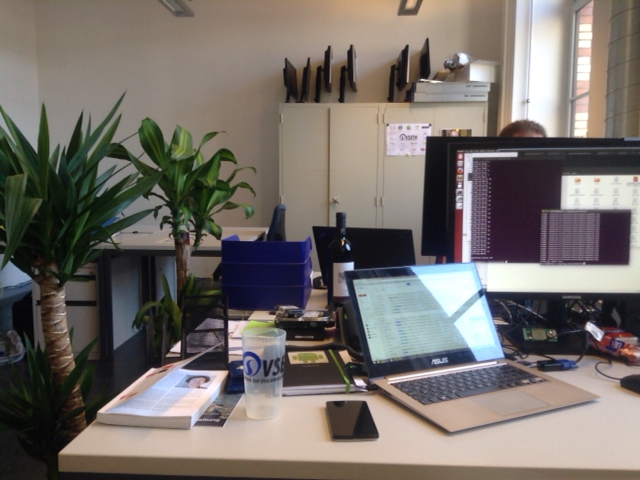
\includegraphics[width=\textwidth]{figures/color1}
				\caption{Color image}
				\label{fig:color1}
			\end{subfigure}
			~
			\begin{subfigure}[b]{0.3\textwidth}
				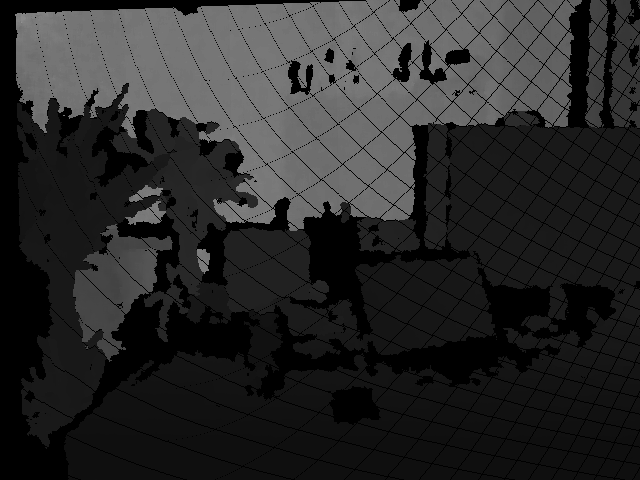
\includegraphics[width=\textwidth]{figures/mapped1}
				\caption{Re-projected depth}
				\label{fig:mapped1}
			\end{subfigure}
			\caption{Comparison between recorded depth and re-projected depth frame}
		\end{figure}
		
		Because we project the depth values into the color frame we lose some information. E.g. the values which would be projected outside the color frame can't be used anymore, for that reason the back-projected depth frame has black borders. We also see some aliasing effects throughout the entire image which is a sampling problem. This could be solved by a triangulation approach.

		\begin{figure}[h]
			\centering
			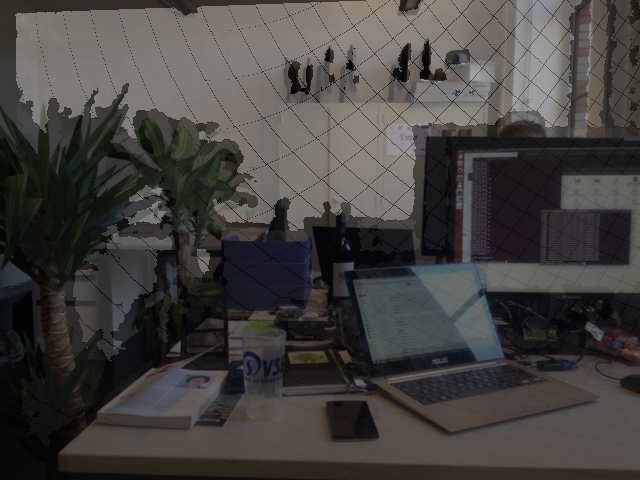
\includegraphics[width=0.75\textwidth]{figures/both}
			\caption{RGB-D pair as a 4-channel image}
			\label{fig:rgbd}
		\end{figure}	
	
\chapter{3D Reconstruction}
	The first step of the 3D reconstruction is to obtain the camera trajectory. For this matter we use a semi-direct motion estimation approach. This pipeline will be slightly extended to output some more results which will be used in the scale estimation step. Due to the fact that the motion estimation is only based on color images we need a scaling step to correct the discrepancy between the absolute metric of the depth map and the relative coordinates of the motion estimation. The final step is to perform the volumetric 3D mapping and texturing which is done by the Fastfusion pipeline.

	\section{Camera Tracking - SVO}
		For the camera trajectory estimation Semi-Direct Monocular Visual Odometry \cite{svo} (SVO) is used. This is a pipeline that implements motion estimation in a semi-direct fashion. It uses two parallel threads, one for estimating the camera motion and the second for mapping. 
		
		The motion estimation thread implements the semi-direct approach, which means that it estimates motion directly form intensity values, instead of using robust feature matching as in non-direct approaches. In the first step it initializes the camera pose based on sparse model-based image alignment, it minimizes the photometric error between pixels of different frames projecting to the same 3D location. Then feature-patches are aligned to refine the 2D coordinates of the reprojected points. Finally pose and structure are refined by minimizing the reprojection error introduced in the feature alignment step.
		
		The mapping thread initializes a probabilistic depth-filter for every 2D feature for which the corresponding 3D is to be estimated. When a new keyframe is selected in regions of the image with few 3D to 2D correspondences, new depth-filters are initialized. The filters are initialized with a large uncertainty in depth and then updated at every subsequent frame until its uncertainty becomes small enough, whenever a new 3D point is inserted in the depth map.
		
		As mentioned before the pipeline is extended, it also outputs the $(u,v)^T$ coordinates and the corresponding $Z$ coordinate of every tracked feature. In other words, we obtain the 2D feature's coordinates and the estimated depth. Unchanged is the rest of the pipeline which outputs the camera pose for every frame. 
		
		Several challenges needed to be overcome when using the SVO pipeline, because there were several datasets where no camera poses could be estimated. On one side it was discovered that the device movement largely impacted the performance of SVO. Because of compatibility reasons depth maps were saved as XML files on the iPad which strongly influenced the frame rate at which datasets could be recorded. Thus moving the camera and sensor slowly and steady was required. On the other hand good lighting conditions and a complex scene were also crucial to get good results. The preceding point is especially important because the quality of the recorded image was not high (VGA). Hence higher resolution images could improve the results but might need better hardware.
		
%	\section{Camera tracking - bundler / visualsfm}
%		Operates with sift, no consecutive frames, matches all images. Takes longer, but also bad performance
	
	\section{Scale Estimation}
		Up to this point we know the camera pose for every frame and the coordinates of the tracked features over all frames. The arising problem is that the estimated 3D coordinates of the features are in a coordinate system with a relative scale. On the other hand the depth values recorded by the structure sensor are saved based on an absolute scale, in millimeters. This means that the relative coordinates must be scaled to match the absolute coordinates.
		
		Thus for a feature at position $(X,Y,Z)^T$ which is projected to $(z_iu_i,z_iv_i,z_i)^T$
		in the camera frame, $z_i$ usually doesn't equal the $z$ value of $P_{rgb}$ in \ref{eq:Prgb}, here denoted as $d_i$. Therefore we need to introduce a scale factor which corrects the depth difference. We used a simple least squares approach to approximate s:
		
		\begin{equation}
			\sum_{i=0}^{pixels \cdot images} (d_i - s\cdot z_i)\cdot z_i = 0
		\end{equation} 
		
		Subsequently we scale every camera pose by the factor $s$. Because the camera pose is computed by
		\begin{equation}
			\label{eq:camera_center}
			c_j = -R_j^T\cdot t_j
		\end{equation}
		where $c_j$ is the camera center of the $j$'th camera and $[R_j|t_j]$ is the camera to world coordinate system transformation matrix. Therefore it is enough to scale the vector $t_j$ by a factor of $s$ to account for the wrong depth.
		
	\section{Pointcloud}
		To obtain  a visual confirmation that the scale estimation succeeded, the RGB-D pairs were converted to pointclouds. The model from \ref{eq:model} is used along with the camera intrinsics to project to the camera coordinate system. Then the rotation and the translation of the camera pose are used as extrinsic parameters and the image is projected to the world coordinate system. Equation \ref{eq:model_inv} shows how the pinhole model of \ref{eq:model} is used in reverse.
		
		\begin{equation}
			P_i = R_{rgb}^{T}(K_{rgb}^{-1}p_i - t_{rgb})
			\label{eq:model_inv}
		\end{equation}
		where $p_i$ is the vector 
		$(u_{i}d_{i},v_{i}d_{i},d_{i})^T$.
		Here $u$ and $v$ are the pixel coordinates in the color camera frame with depth $d$ in the depth frame.
		Accordingly the color of pixel $p_i$ with depth $d$ is the RGB value at $(u_i,v_i)^T$.
		
		\begin{figure}[h]
			\centering
			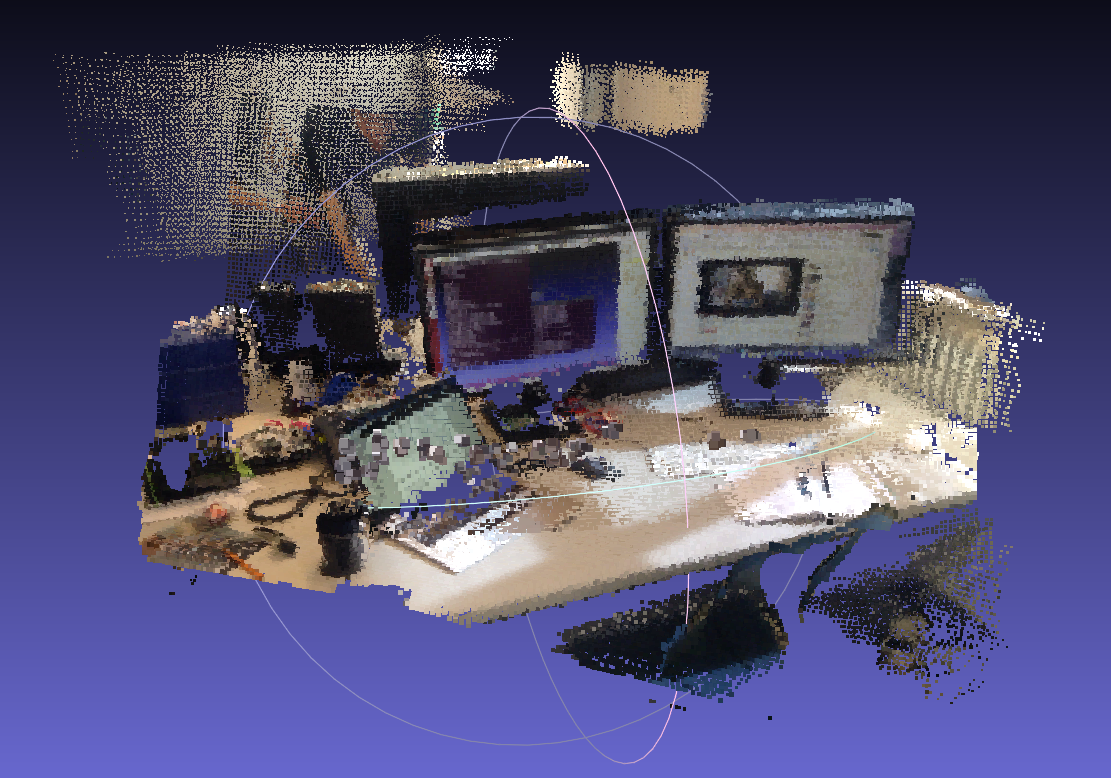
\includegraphics[width=0.75\textwidth]{figures/ptcl1}
%			\caption{Re-projected depth image}
			\label{fig:pointcloud1}
		\end{figure}
		
		\begin{figure}[h]
			\centering
			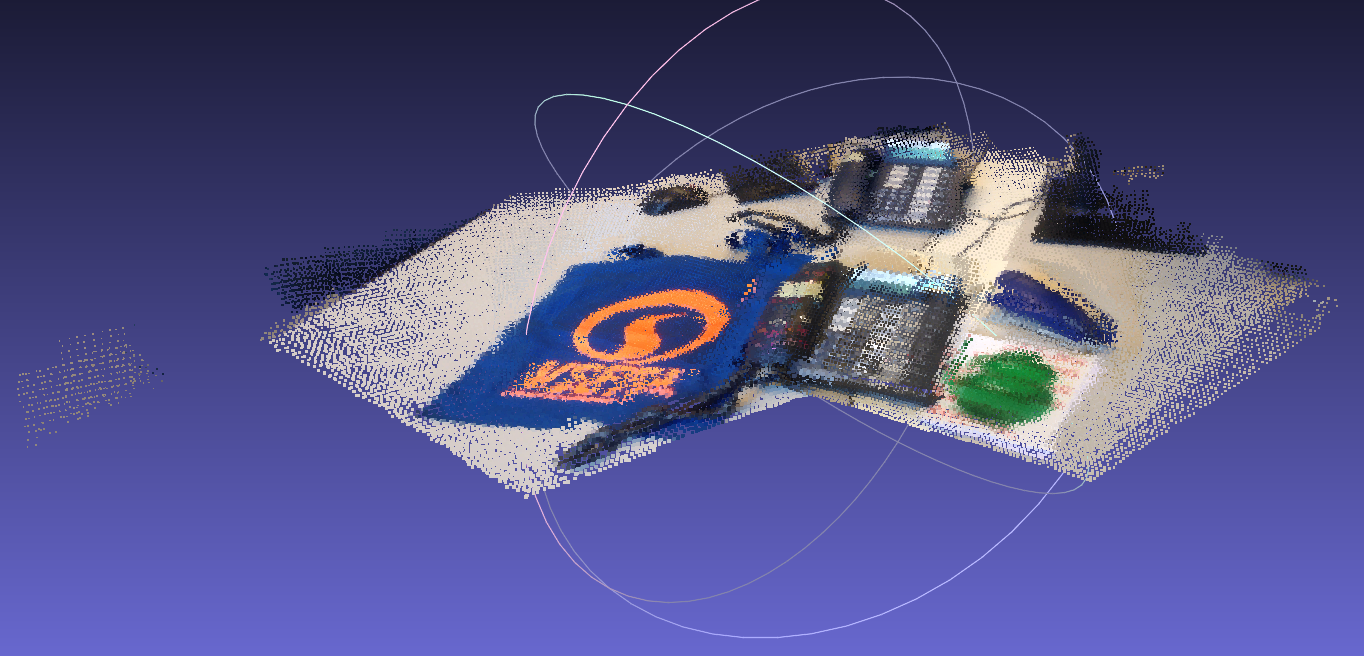
\includegraphics[width=0.75\textwidth]{figures/ptcl2}
			\caption{Pointclouds visualized in MeshViewer}
			\label{fig:pointcloud2}
		\end{figure}
		
	
	\section{Dense Reconstruction}
		The final step of the reconstruction process is the volumetric mapping. Here the Fastfusion \cite{fastfusion} pipeline is used because it doesn't need a special sensor, as the Kinect Fusion, thus works with our data. Furthermore it runs on the CPU and doesn't need any special GPU, hence it can be run on any desktop computer or laptop.
		
		Fustfusion uses an octree data structure to perform the volumetric meshing and mapping. Moreover it incorporates two different algorithms, the first for data fusion and the second for incremental meshing, each running in their own thread.  The geometry of the reconstruction is represented using a signed distance function (SDF) which is saved in an octree. This choice was made because usually most of the space is either free or unknown. The octree is then able to save different distances at different levels in the tree, thus obtaining several resolutions. In the visualization the highest resolution is used and the lower resolutions serve as fallback. Furthermore every node in the tree contains a small cubic volume called brick which itself contains $8^3$ voxels. Lastly the voxel stores the distance, weight and color of a point.
		
		In the fusing process the algorithm iterates over all pixels in an image, computes its 3D point and looks up its corresponding brick in the tree. Upon that the distance value in every concerning brick is updated. In the next step the geometry representation as an SDF needs to be converted to a triangle mesh. This type of storage is better because of a lower memory footprint. Here the Marching Cubes algorithm is applied and mesh cells are created which are associated with branches in the tree.
		
		The challenges which were to overcome when using Fastfusion were mostly about the data format. For example the image scale needs to be specified, since the default scale is 5000 (1 millimeter is multiplied by 5000), we chose to also use this format, thus every depth frame needed to be converted accordingly. Moreover the pipeline takes the camera center as in \ref{eq:camera_center} and the camera rotation as input. Unfortunately this was not clearly specified, besides the rotation needed to be inverted first which resulted in some confusion.
		
		\begin{figure}[h]
			\centering
			\begin{subfigure}[b]{0.8\textwidth}
				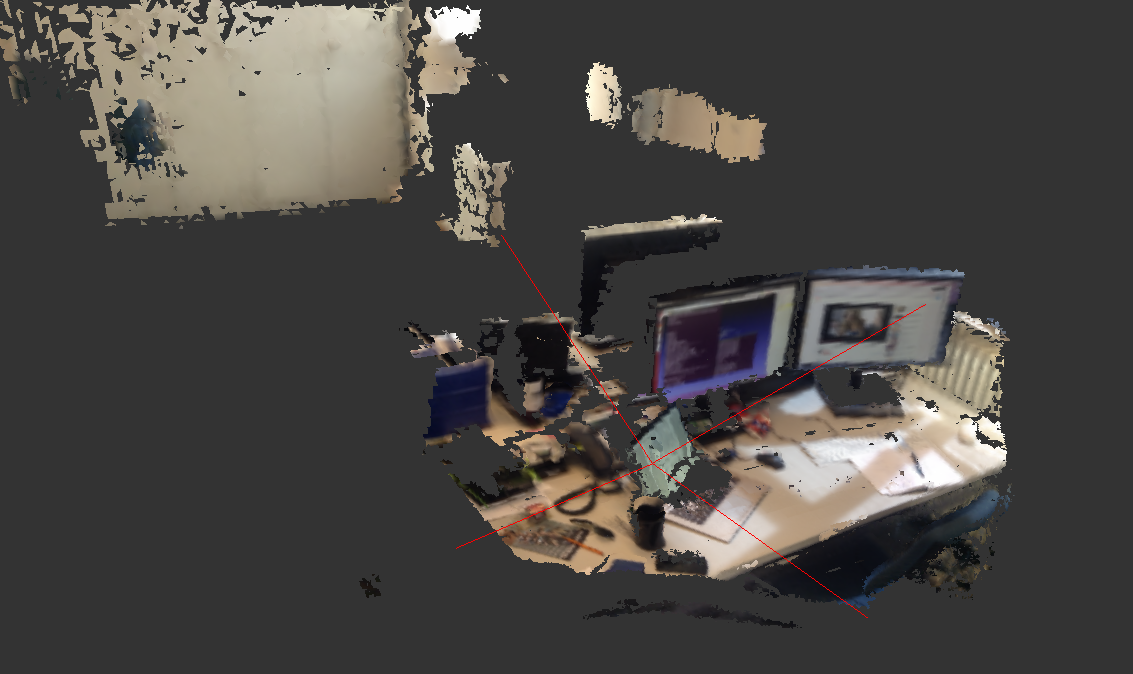
\includegraphics[width=\textwidth]{figures/recon1}
				\caption{Desk scene front view}
				\label{fig:recon11}
			\end{subfigure}
			\begin{subfigure}[b]{0.8\textwidth}
				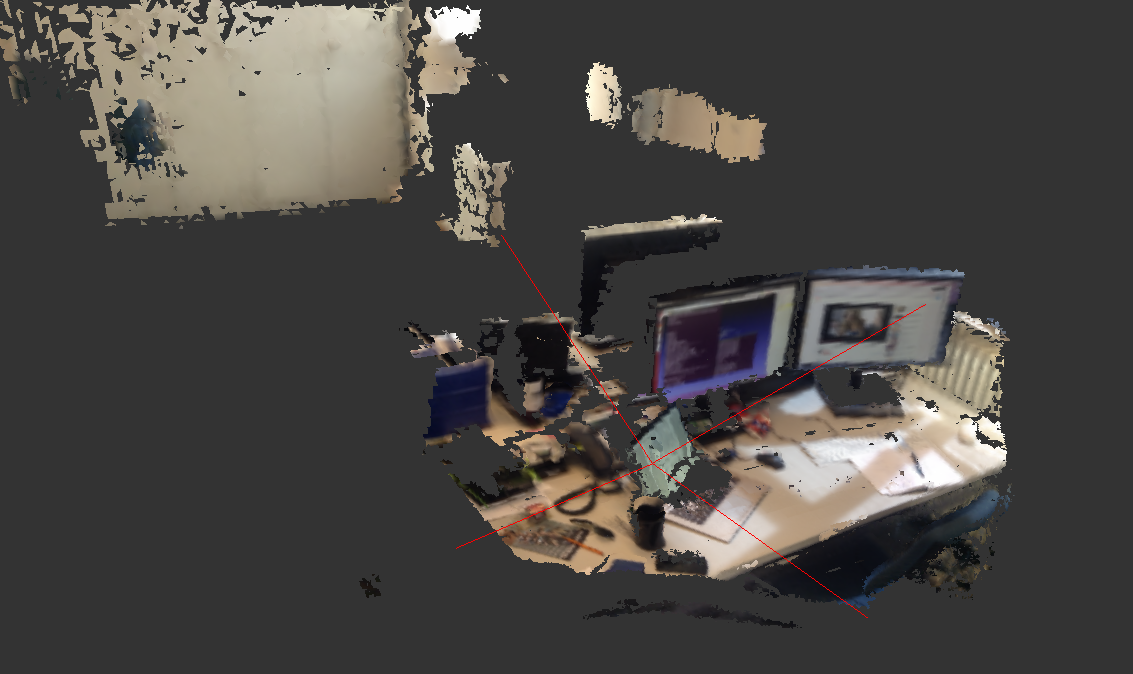
\includegraphics[width=\textwidth]{figures/recon1}
				\caption{Desk scene front view}
				\label{fig:recon11}
			\end{subfigure}		
			\begin{subfigure}[b]{0.8\textwidth}
				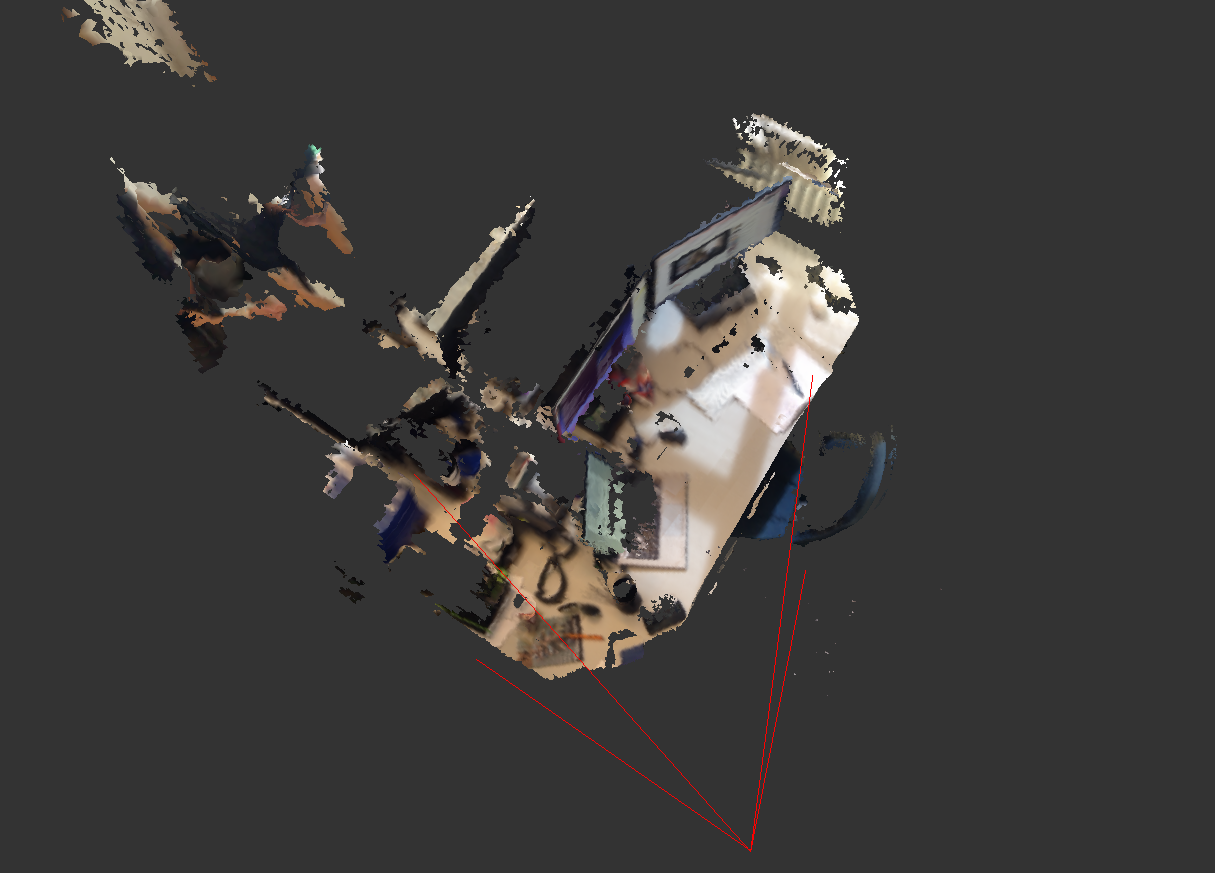
\includegraphics[width=\textwidth]{figures/recon11}
				\caption{Desk scene from above}
				\label{fig:recon12}
			\end{subfigure}
			\caption{reon1}
		\end{figure}
		
		\begin{figure}[h]
			\centering
			\begin{subfigure}[b]{0.8\textwidth}
				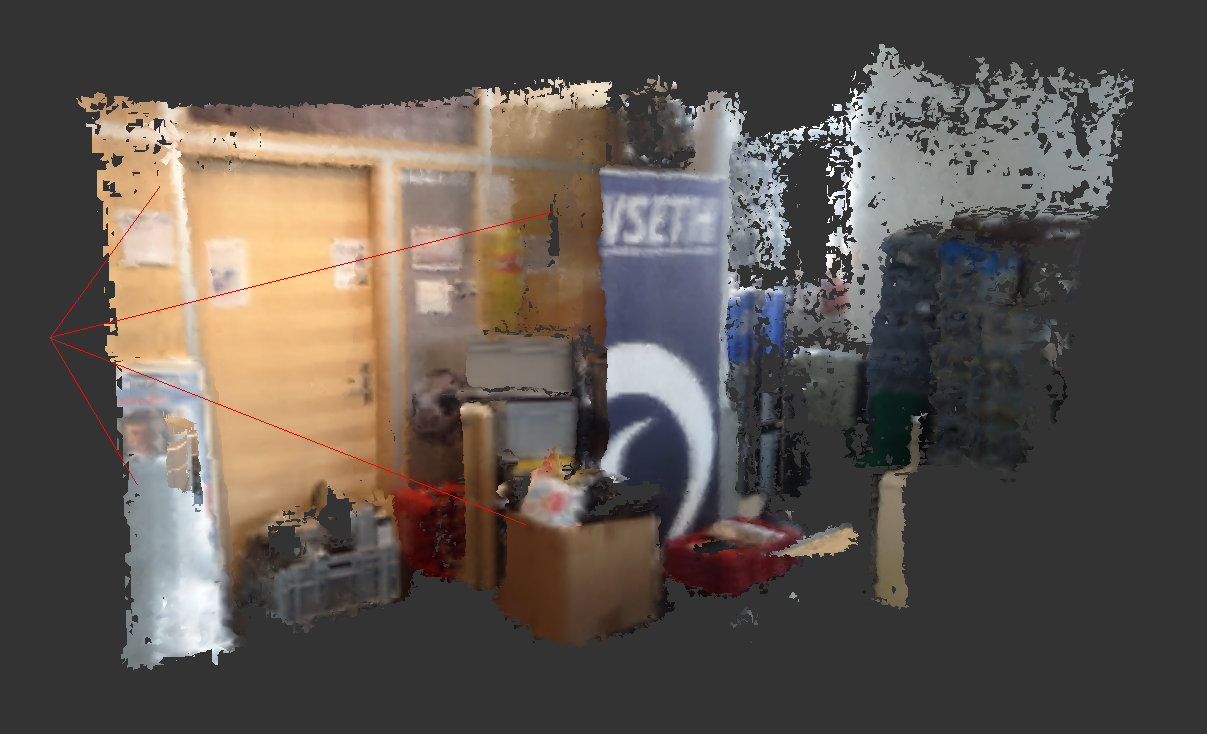
\includegraphics[width=\textwidth]{figures/recon2}
				\caption{Room front view}
				\label{fig:recon21}
			\end{subfigure}
			\begin{subfigure}[b]{0.8\textwidth}
				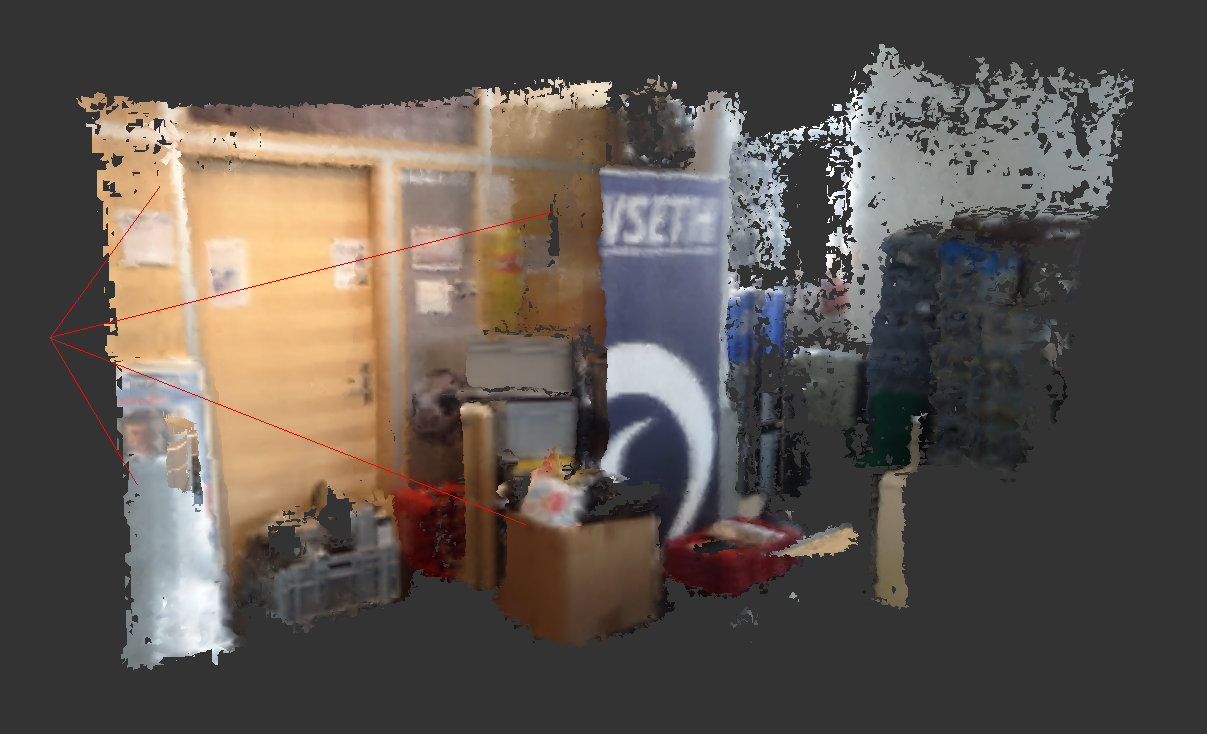
\includegraphics[width=\textwidth]{figures/recon2}
				\caption{Room front view}
				\label{fig:recon21}
			\end{subfigure}
			\begin{subfigure}[b]{0.8\textwidth}
				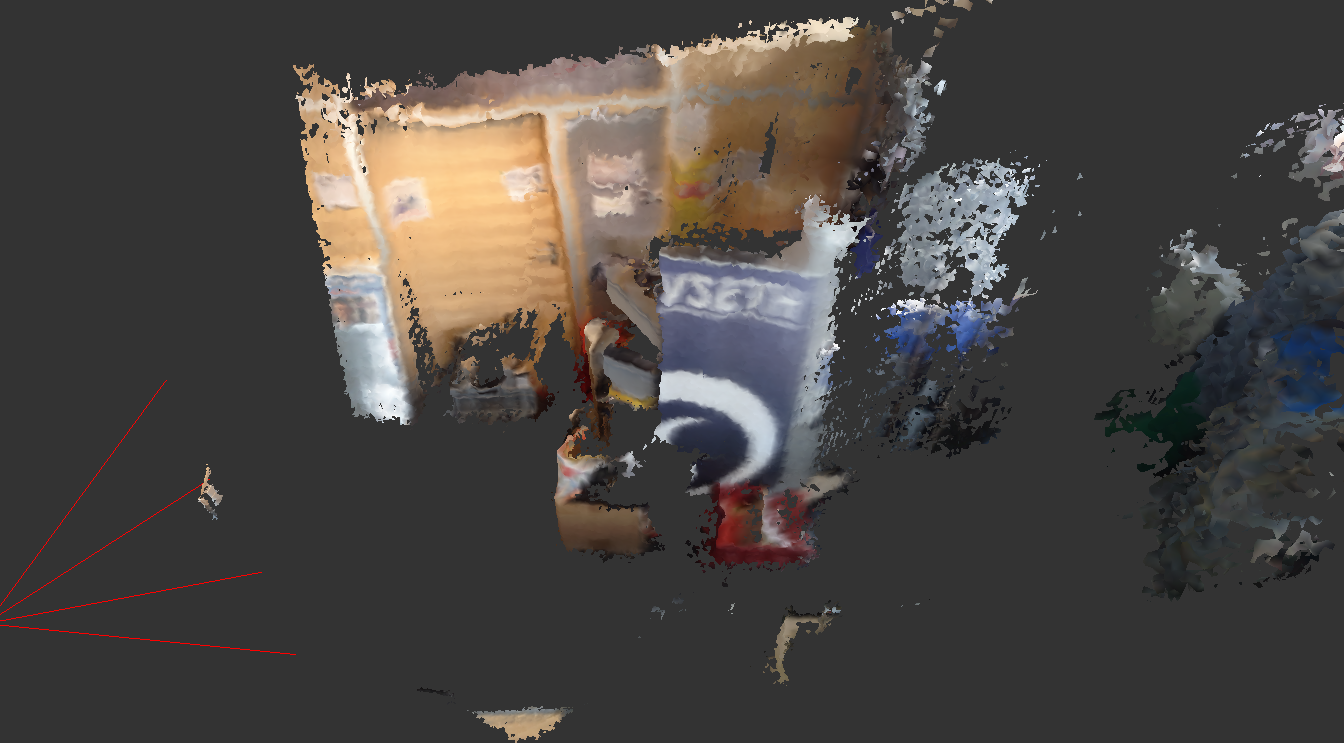
\includegraphics[width=\textwidth]{figures/recon22}
				\caption{}
				\label{fig:recon22}
			\end{subfigure}
			\caption{reon1}
		\end{figure}	
		
		\todo{new images}

\chapter{App integration}
		
			
			
\chapter{Conclusion}

	The original idea of this thesis was to obtain data from the Structure sensor on a mobile device, calibrate the sensor and the camera to be able to combine the two inputs and finally perform a 3D reconstruction. Additional ideas were to add model fitting or some body pose estimation and extract the skeleton. And there was the possibility to integrate the depth acquisition process into the application of \cite{paper1}. 
	
	Whereas we were not able to acquire data on an Android device this worked smoothly on iOS devices due to the available development kit. The main challenge was to extract the recorded data from the device. Especially for the depth frames this was harder then expected because iOS has a different data security model than Android and doesn't allow export of every data format as easily. The resulting workflow of how to transfer the recorded data from the mobile device to the desktop device showed to be easy but could be improved by using a cloud storage or by an all on device approach as described in \ref{ch:future}.
	
	The calibration step was first done offline and then ported to the mobile device. Fortunately this worked quite well, the on device calibration has the advantage that the application can easily be run on different devices and there is no additional configuration work to be done offline. Furthermore it has the advantage that the sensor can be moved arbitrarily between different recordings and only a quick two step calibration needs to be performed to update the configuration. Next, the depth re-projection proofed to be more cumbersome. First there were different challenges with the algorithm itself, like using the closest depth or eliminating the points which projected outside the image plane. Then re-projecting on the device didn't work, at least not real-time, for performance reasons. So this step needed to be performed offline which is unfortunate in particular with regard to the all on device approach. 
	
	Regarding the 3D reconstruction pipeline we note that the original intention was too optimistic. This step showed to be the most challenging and time consuming. Originally the dense visual odometry pipeline should have been used because it conforms with the Fastfusion pipeline. Due to the fact that this pipeline was running on ROS\footnote{Robot Operating System} the usability was hindered. Therefore it was decided to use SVO instead, the drawback being that the camera motion estimation solely relies on color images and not on depth information.  As a result the camera motion was estimated in some arbitrary coordinate system, whereas the depth coordinates are stored in millimeters. Therefore scaling must be performed. The approach taken compares the estimated depth values with the real depth and computes an averaging scaling factor. This is then applied to the camera center translation, in practice this proofed to be accurate enough and good results could be obtained. The other drawback of using SVO was that it doesn't work as well in less textured environments. Thus care must be taken when choosing scenes.
	
	The additional tasks like model fitting and body pose estimation were left out because time constraints would not have allowed a profound commitment to the matter. Instead the application described in \cite{paper1} was made available in iOS and the depth data acquisition could be integrated. This integration nicely completed this work on depth sensors on mobile devices and allowed to show the practicality of mobile depth sensors by enhancing the current application.
	
	Conclusively I can wind up that the original objectives could not all be obtained due to unforeseen challenges and maybe too ambitious prospects. On the other hand different approaches have been tried and therefore and in general a lot about the matter has been learned. Besides, especially the integration of the sensor in an existing application encouraged the enthusiasm for further projects in the field.  


\chapter{Future work}
\label{ch:future}

	In this chapter we describe possible future work or extensions to this project. Suggestions are based on efforts which didn't succeed, like for example the Android version. Also tasks which were out of scope because of time constraints will be addressed.
	
	At first we wanted to use Android as platform for the Structure sensor. The problem at the time was that not many devices supported USB host mode which was necessary for the sensor to communicate with the mobile device. Now that more devices support the feature it would be worth to work on data acquisition for Android devices again. The other problem with Android was that the integration with OpenNI and the NDK platform proved to be cumbersome, in the future where Occipital is supposed to release additional resources for Android this could also be solved.
	
	The second point concerns the pipeline. For usability reasons it would be great to have it in one application which runs on a mobile device. Therefore the data acquisition and camera calibration could be combined with a mobile visual odometry or a dense visual odometry approach. This could then be extended to also feature mobile reconstruction. In an next step consumer feature could also be added like measuring in the reconstruction or export to 3D file formats to be able to print the recorded object.
	
	An extension to the project which we didn't have time for is model fitting. In the present state everything seen by the camera and sensor is recorded and reconstructed. Still there are cases where you actually only want to record a subset of the viewed scene, e.g. if the background is irrelevant and can be discarded. For that reason we propose to integrate model fitting into the application. The first possibility is to perform a 2D model fitting and then only track and reconstruct the matched region. Another more robust approach is to do 3D model fitting. This has the advantage that there are less features required, thus it works better in less textured environments.  
	
	
%And here we cite an external document~\cite{TestReference}.

% This displays the bibliography for all cited external documents. All references have to be defined in the file references.bib and can then be cited from within this document.
\bibliographystyle{splncs}
\bibliography{references}

% This creates an appendix chapter, comment if not needed.
\appendix
\chapter{Code}

	\section{Depth Re-projection}
		\label{ap:reprojection}
		\begin{lstlisting}
for (int row = 0; row < depthRaw.rows; ++row) {
	for (int col = 0; col < depthRaw.cols; ++col) { 
		
		// get depth for re-projection
		double depthVal = (double)ptrOrig[depthRaw.cols*row + col];
		
		// Map depthcam depth to 3D point
		Mat_<double> P3D = Mat_<double>(3,1);
		
		P3D(0) = (col - camera1.at<double>(0,2)) 
		* depthVal / camera1.at<double>(0,0);
		P3D(1) = (row - camera1.at<double>(1,2)) 
		* depthVal / camera1.at<double>(1,1);
		P3D(2) = depthVal;
		
		// Rotate and translate 3D point
		Mat_<double> P3Dp;
		P3Dp = (R*P3D) + T;
		
		// Project 3D point to rgbcam
		double xrgb = (P3Dp(0) * camera2.at<double>(0,0) / P3Dp(2)) 
		+ camera2.at<double>(0,2);
		double yrgb = (P3Dp(1) * camera2.at<double>(1,1) / P3Dp(2)) 
		+ camera2.at<double>(1,2);
		double nDepth = P3Dp(2);  
		
		// "Interpolate" pixel coordinates (Nearest Neighbors)
		int px_rgbcam = cvRound(xrgb);
		int py_rgbcam = cvRound(yrgb);
		
		// Handle 3D occlusions
		uint16_t &depth_rgbcam = 
		ptrMapped[depthRaw.cols * py_rgbcam + px_rgbcam];
		uint16_t &depth_rgbcamScale = 
		ptrMappedScale[depthRaw.cols * py_rgbcam + px_rgbcam];
		
		if(px_rgbcam - depthRaw.cols < 0 
		&& py_rgbcam - depthRaw.rows < 0) {
			if(depth_rgbcam == 0 || (uint16_t)nDepth < depth_rgbcam) {
				depth_rgbcam = 5*(uint16_t)nDepth; //scale by 5 for fastfusion
			}
		}   
	}
}
		\end{lstlisting}

\end{document}